\documentclass[12pt, authoryear]{elsarticle}
\makeatletter
\def\ps@pprintTitle{%
	\let\@oddhead\@empty
	\let\@evenhead\@empty
	\def\@oddfoot{}%
	\let\@evenfoot\@oddfoot}
\makeatother
%\usepackage{lmodern}
% My spacing
\usepackage{setspace}
\setstretch{1.5}
\usepackage{multirow}
%\DeclareMathSizes{12}{14}{10}{10}
\usepackage[margin=2.5cm]{geometry}    % How to set margins - optimized for 2.5cm      

% See geometry.pdf to learn the layout options. There are lots.
\geometry{a4paper}                   			% ... or a4paper or a5paper or ... 
\usepackage{enumitem}
\usepackage{mathtools}
%\geometry{landscape}                		% Activate for rotated page geometry
\usepackage[parfill]{parskip}    			% Activate to begin paragraphs with an empty line rather than an indent
\usepackage{graphicx}						% Use pdf, png, jpg, or eps§ with pdflatex; use eps in DVI mode
% TeX will automatically convert eps --> pdf in pdflatex	
\usepackage{flafter}			
\usepackage{setspace}
%\linespread{1.5}
\usepackage[font={}]{caption}
\usepackage[bottom]{footmisc}
\usepackage[capposition=top]{floatrow}   %figure notes
\usepackage{lscape}
%math packages 
\usepackage{amssymb}
\usepackage{fancyhdr}
\usepackage{graphicx,epsf,subfigure}
\usepackage{pstricks,pst-node,psfrag}
\usepackage{amsthm,amssymb,amsmath}
\usepackage{amsmath,bm}

%mathnotes
\newcommand{\bbeta}{\mbox{\boldmath $\beta$}}
\newcommand{\beps}{\mbox{\boldmath $\epsilon$}}
\newcommand{\bX}{\mbox{\boldmath $X$}}
\newcommand{\bY}{\mbox{\boldmath $Y$}}
\newcommand{\bI}{\mbox{\boldmath $I$}}
\newcommand{\N}{\mathcal{N}}
\newcommand{\x}{\textsc{\textbf{x}}}
\newcommand{\xx}{\textsc{x}}

%add figure 
\DeclareGraphicsRule{.tif}{png}{.png}{`convert #1 `dirname #1`/`basename #1 .tif`.png}
\usepackage{rotating}
\usepackage{pdflscape}
\usepackage{hyperref}
\usepackage[round]{natbib}

\usepackage{soul}

\def\bibsection{\section{References}} %%% Make "References" appear before bibliography
\usepackage{longtable}
\usepackage{hyperref}
\usepackage{tablefootnote}
\usepackage{lscape} 
\usepackage{animate}

\renewcommand{\contentsname}{Table of Contents} % change name from Contents to Table of Contents

\usepackage{titlesec}

\setcounter{secnumdepth}{4}

%_______________________________________________________________________________________________________%
%_______________________________________________________________________________________________________%
%\usepackage[table]{xcolor}% http://ctan.org/pkg/xcolor
%\usepackage{graphicx,multirow}
\usepackage{xcolor,colortbl}
\usepackage{xcolor}
%\usepackage{graphicx,multirow}
\usepackage[capposition=top]{floatrow}
\setcounter{secnumdepth}{4}
\usepackage{tikz}
\begin{document}

\begin{frontmatter}  %

\title{AB Testing Totalwatchrepair.com}

\author[Add1]{Reid Falconer}
\ead{reid.falconer@bracelonagse.eu}

\author[Add1]{Eric Beckwith}
\ead{eric.beckwith@bracelonagse.eu}

\author[Add1]{Felix Adam}
\ead{felix.adam@bracelonagse.eu}
\author[Add1]{Maryam Rahbaralam}
\ead{maryam.rahbaralam@bracelonagse.eu}

\address[Add1]{Barcelona Graduate School of Economics, Barcelona, Spain}
%\address[Add2]{Some other Institution, Cape Town, South Africa}

%\cortext[cor]{Corresponding author: Nico Katzke}

%\begin{abstract}
%\small{
%Abstract to be written here. 
%}
%\end{abstract}

%\vspace{1cm}

%\begin{keyword}
%\footnotesize{
%Demand Estimation \sep A/B Testing \sep  \\ \vspace{0.3cm}
%\textit{JEL classification} L250 \sep L100
%} 
%\end{keyword}
%\vspace{0.5cm}
\end{frontmatter}

\headsep 35pt % So that header does not go over title
\section*{AB Testing Totalwatchrepair.com}\label{ab_testing}

\subsection*{Business Model}
Totalwatchrepair.com is a company specialising in mail-order watch repairs. Their business is centred around providing servicing for high-quality mechanical watches such as Rolex and Breitling.  Customers have the opportunity to request free estimates and then send in their timepieces by mail. The company then provides an initial assessment of repairs to be made. If the customer agrees to the proposal, all necessary services will be performed, and the watch will then be sent back to the customer through the mail. 

Amongst the services provided by totalwatchrepair.com are simple tasks such as crown- and crystal replacement as well as highly technical jobs such as complete mechanical overhauls and restorations. 

The business model of totalwatchrepair.com relies upon receiving requests for watch repairs. The focus of their online-appearance should, therefore, be on encouraging visitors to send a request to the company. Their secondary business model is selling accessories, most notably replacement watch straps. Given these two sources of revenue, we propose improvements to the website which should ultimately help increase total revenue.

\subsection*{Increased Requests}
As of now, the landing page has the following layout:

\begin{figure}[!htp]
	\centering
	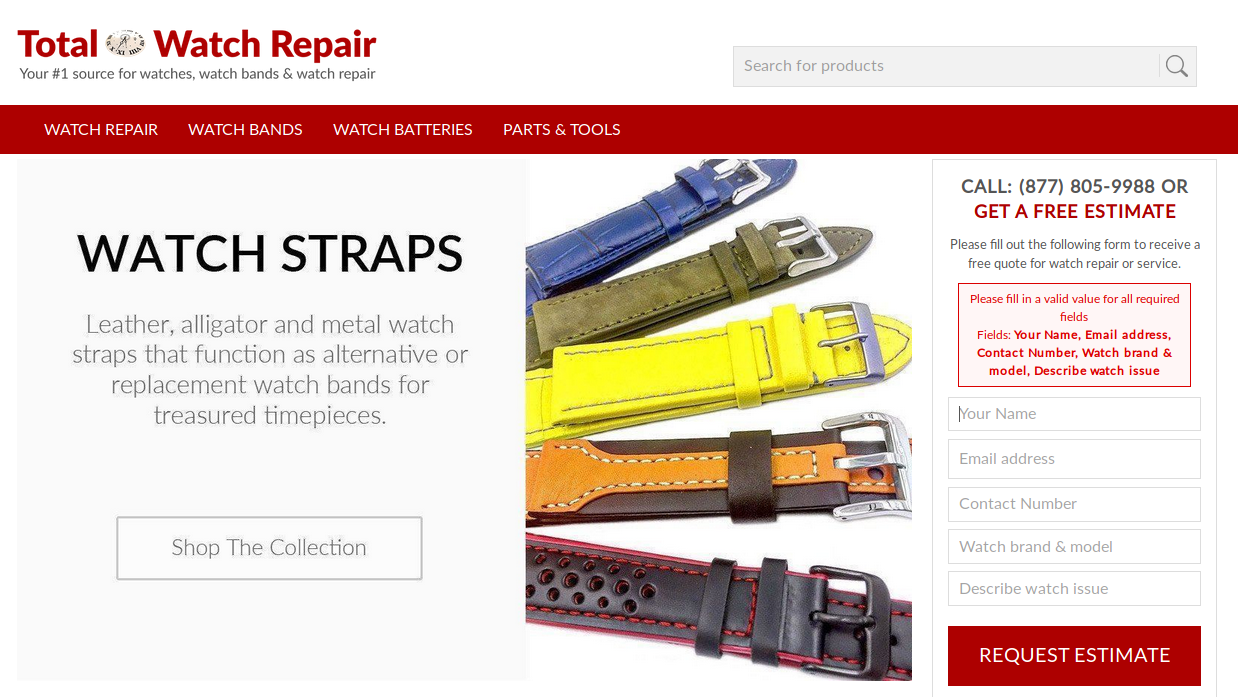
\includegraphics[clip, angle=0,width=0.8\textwidth]{LandingPage.png}
	\caption{ Current Landing Page}\label{LandingPage}
\end{figure}

Visitors arriving on the page can click on the red ‘Request Estimate’ button. However, without filling out the form, they will receive an error message as shown in \ref{LandingPage}. Some customers may find this form to be daunting or are unwilling to make this initial `commitment' right away.  Also, currently clicking on the red button without filling in the form results in an error message.

\textbf{Proposal:} Remove the form and leave the request estimate button with the phone number. When the user clicks on `Request Estimate' she is being lead to the next page where the form can be filled out.

\begin{figure}[H]
	\centering
	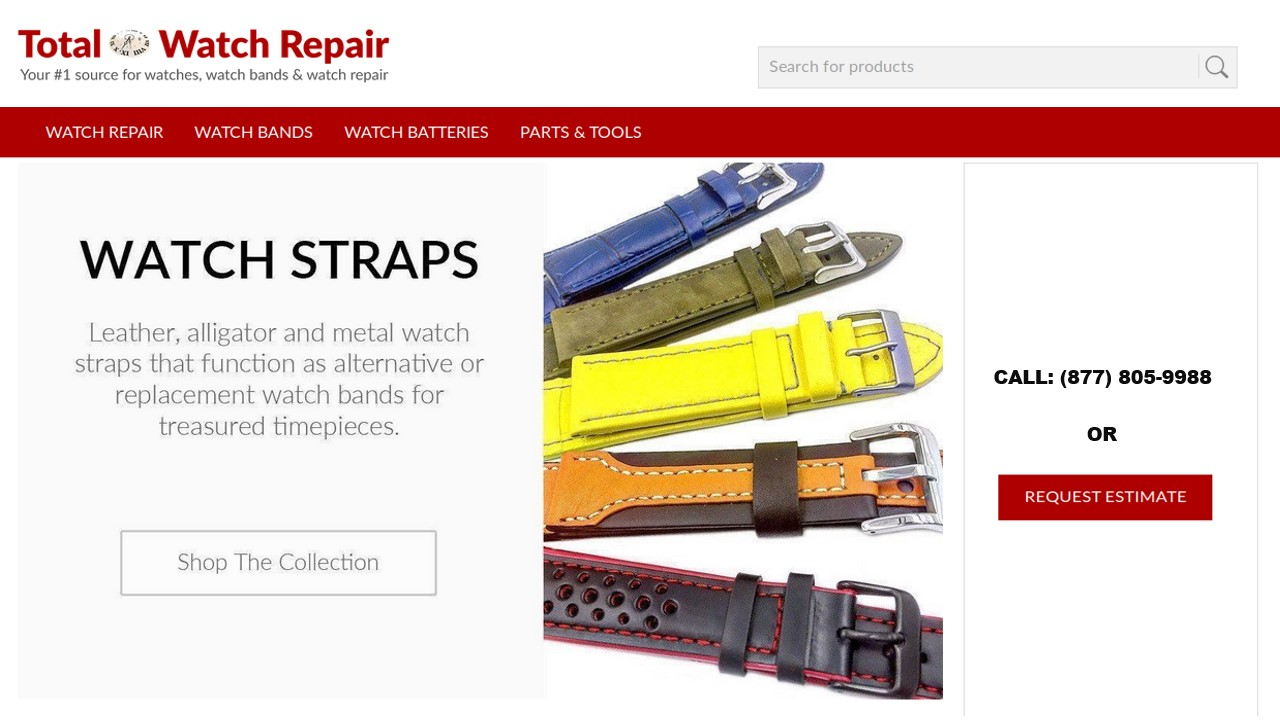
\includegraphics[clip, angle=0, width=0.8\textwidth]{New_Landing_Page.jpg}
	\caption{Proposed Landing Page}\label{NewLandingPage_Shop}
\end{figure}

\textbf{Hypothesis 1}: The new page design will result in an improved form submission rate when compared to the current design.

Ultimately, our goal is to improve the form submission rate, since this could potentially lead to more accepted offers and increased revenue. However, we would also like to track the click-through rate on our new button structure compared to the original website.

If we have succeeded in getting more customers to click through to the estimate page, yet they are still not submitting forms, this is valuable information as well - we can then potentially look at a second stage where we make alterations to the form submission page.

Submission rate represents the percentage of visitors who enter the site and submit a completed form while the click rate is the percentage of people who click the red button in either instance. We believe that for this website we can randomise the population that sees each form, in a 50/50 split. By focusing on form submissions, we are dealing with statistics that likely have a very low current baseline rate for all visitors.  Because of this, we do not need an overly large sample to get a relatively powerful test. While we believe that a 5 per cent significance level would suffice for this test, an argument could be made for a smaller level of significance since the cost of testing is relatively low and this is far from a time-sensitive business where the length of testing time is a major concern. Furthermore, we assume that the baseline conversion rate for form submissions is relatively low, presumably around 3\% based on contact form submission averages. 

Therefore, we do not need a large number of samples to have good test power. As a simple example, if we assume a Bernoulli distribution for submission and a null hypothesis probability of 0.03.  Then, if we have a population of 500, the expected conversions would be 15, and at a significance level of 0.05, a change of at least 4 would be significant. (see https://www.impactbnd.com/blog/what-is-a-good-landing-page-conversion-rate for a complete explanation of the chosen statistics). 

A potential bias with this testing structure could arise from the fact that the phone number is more exposed. Customers could now be inclined to call more, which would ultimately lead to a reduced number of filled in forms. A potential remedy would be to either change the phone number displayed to the treatment group and then compare the call rates across groups or to exploit some alternative data sources (i.e. page views and national call logs) in attempt to construct a counterfactual for what would have happened to the call rate in the absence of the AB test.

\subsection*{Increased Shop Visits}

Currently, the button for the shop the collection is somewhat transparent and not very readable or engaging. To generate sales, more customers should click on the ‘Shop The Collection’ button.  

\textbf{Proposal:} Make a button that stands out more and fits the overall theme of the website:

\begin{figure}[H]
	\centering
	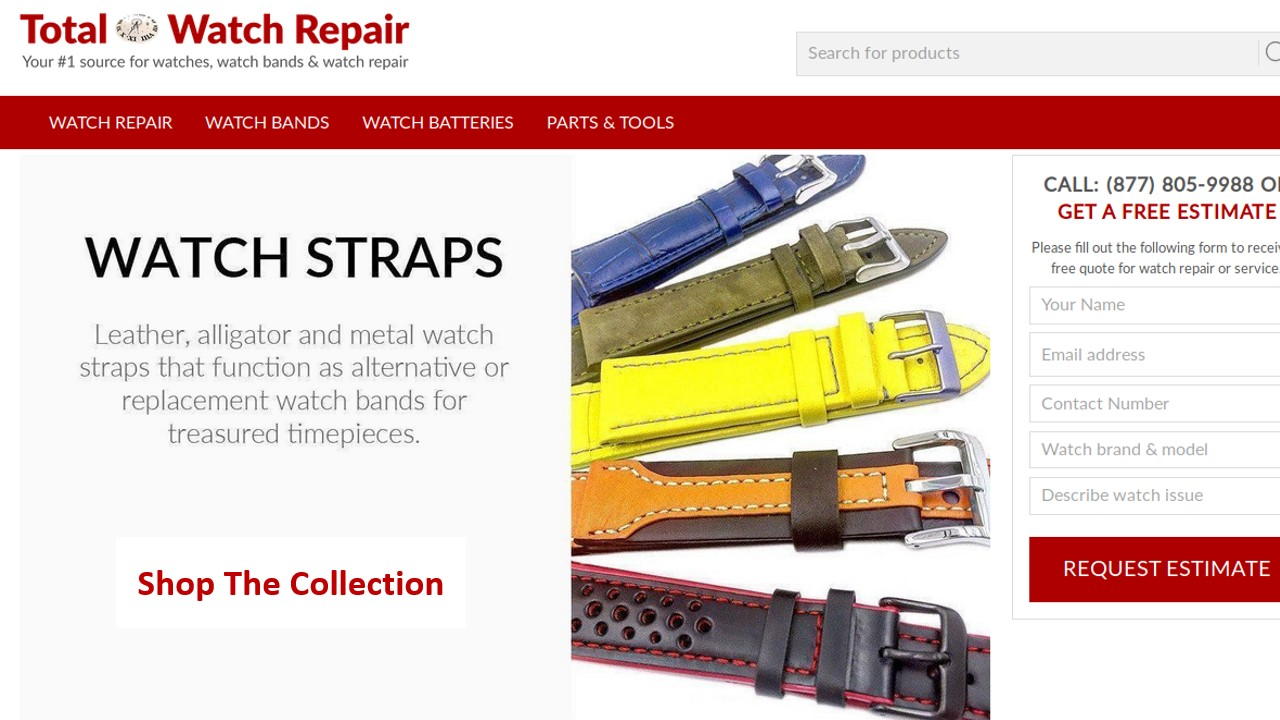
\includegraphics[clip, angle=0, width=0.8\textwidth]{New_Shop_Button.jpg}
	\caption{New Shop Button}\label{NewLandingPage}
\end{figure}

\textbf{Hypothesis 2}: The new red button has a higher click rate than the old transparent style.

Here we will track the click rate on the new button vs the old style. The click rate represents the percentage of total visitors who click the ‘Shop the Collection’ button in either instance. Again we believe that for this website we can randomise the population that sees each form, in a 50/50 split - though we would ideally run this test independently of Hypothesis 1’s testing. Looking at click rates, which have a higher general baseline rate, means we need a higher number of samples to obtain a similar power to our first test.  We believe that a 5\% level of significance is adequate for this test, as in this case, we would like the testing to be somewhat faster so we can continue to test other alternatives. Further, we would suggest running the test until we have a population size equivalent to a power level of around 80\%, depending on our baseline click rate.

\end{document}
